\begin{figure}[htbp]
\centering
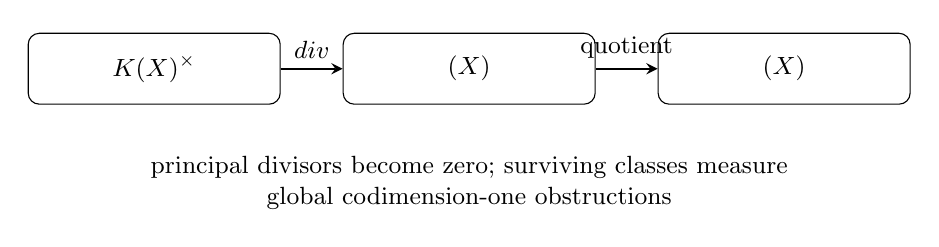
\begin{tikzpicture}[>=stealth,every node/.style={font=\small}]
\node[draw,rounded corners,minimum width=3.2cm,minimum height=.9cm] (k) at (-4,0) {$K(X)^\times$};
\node[draw,rounded corners,minimum width=3.2cm,minimum height=.9cm] (d) at (0,0) {$\Div(X)$};
\node[draw,rounded corners,minimum width=3.2cm,minimum height=.9cm] (c) at (4,0) {$\Cl(X)$};
\draw[->,thick] (k)--node[above] {$\operatorname{div}$} (d);
\draw[->,thick] (d)--node[above] {quotient} (c);
\node[align=center] at (0,-1.45) {principal divisors become zero; surviving classes measure\\global codimension-one obstructions};
\end{tikzpicture}
\caption{The divisor class group is the quotient of Weil divisors by the relations supplied by rational functions.}
\label{fig:vi41-roadmap}
\end{figure}
